
\begin{frame}{Where is Kotlin}
	\begin{columns}
		\begin{column}{0.5\textwidth}
			\onslide<2->{
				\begin{figure}
					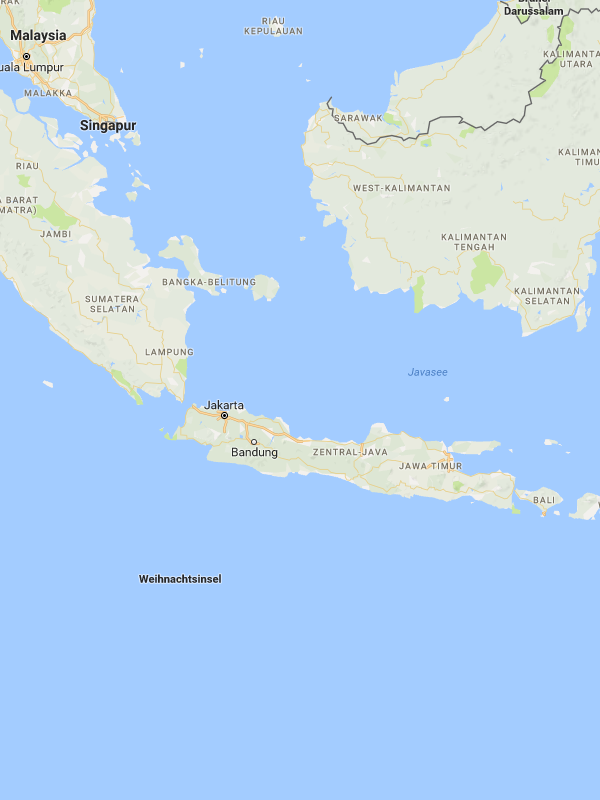
\includegraphics{figures/java}
					\caption{Java}
				\end{figure}
			}
		\end{column}
		\begin{column}{0.5\textwidth}
			\onslide<3->{
				\begin{figure}
					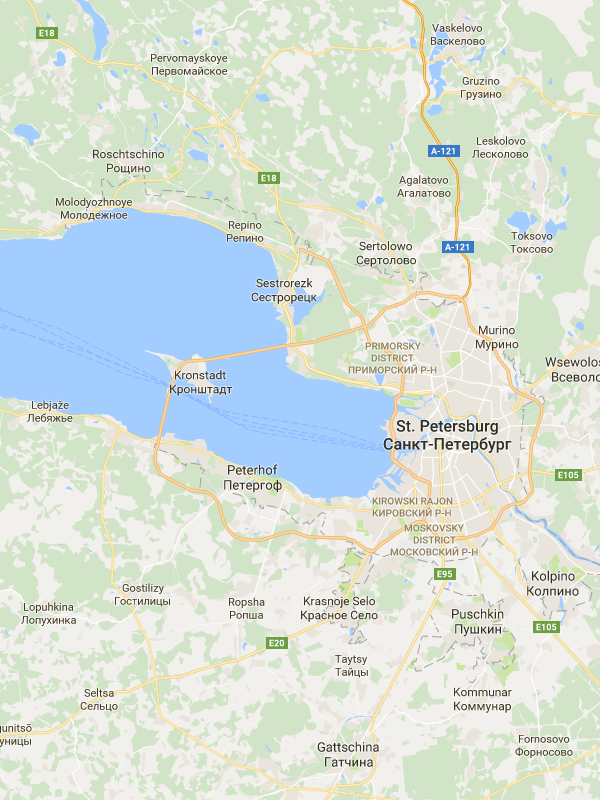
\includegraphics{figures/kotlin}
					\caption{Kotlin}
				\end{figure}
			}
		\end{column}
	\end{columns}
\end{frame}

\begin{frame}{What is Kotlin}
	\begin{itemize}
		\item JetBrains Project - Started 2010
		\item 1.0 Release in February 2016
		\item 1.1 Release in March 2017 (since June: 1.1.3)
		\item 1.2 M1 Release in June 2017
		\item JVM Language (JavaScript and Native in development)
		\item Fast ramp-up
		\item Easy tool-able
		\item Kotlin Standard Library
		\item Small footprint $\leq$ 1MB
		\item Non-Scientific borrow well-established patterns and concepts 
	\end{itemize}
\end{frame}

\begin{frame}{What is Kotlin}
	\begin{itemize}
		\item Java 6 compatible (mobile acceptance)
		\begin{itemize}
			\item Modern features 
		\end{itemize}
		\item Full backward compatibility in minor releases
		\begin{itemize}
			\item Easy and mostly automated migration paths for major releases 
		\end{itemize}
		\item Maven / Gradles support (including useful plugins)
		\begin{itemize}
			\item Kotlin language support for Gradle build scripts
		\end{itemize}
		\item Free Eclipse \& IntelliJ (community) integration
		\item Android support (official since Google I/O 2017)
		\item Spring Boot Kotlin extension (official in Spring 5)
	\end{itemize}
\end{frame}

\section{Key Concepts \& Features}

\begin{frame}{Key Concepts \& Features}
	\begin{itemize}
		\item easy mixing with Java (see samples) \cmark
		\item easy/short idiomatic access (var \& val, getter, setter, data) \cmark
		\item get rid of boilerplate code \cmark
		\item statically typed \cmark
		\item automatically inferred types \cmark
		\item default to closed instead of open classes (+sealed) \tmark
		\item classes \& objects \tmark
		\item nullable? (a billion dollar mistake !!) \cmark
		\item Pairs \& Triples \& Deconstructing \cmark
		\item operator overloading \cmark
	\end{itemize}
\cmark\ \dots\ full sample, \tmark\ \dots\ partial sample, \xmark\ \dots\ no sample
\end{frame}


\begin{frame}{Key Concepts \& Features}
	\begin{itemize}
		\item default to Unit instead of Void as return type \xmark 
		\item lazy properties and delegations \cmark
		\item no checked exceptions \xmark
		\item functional programming (let it lamda) \tmark
		\item higher-order functions \tmark
		\item extension methods \cmark
		\item explicit module system \xmark
		\item runs on android \xmark
		\item can compile to JavaScript \xmark
		\item inlining \& tail recursion \xmark
		\item coroutines \tmark
	\end{itemize}
\cmark\ \dots\ full sample, \tmark\ \dots\ partial sample, \xmark\ \dots\ no sample
\end{frame}

\begin{frame}{Type Hierarchy}
	\begin{columns}
		\begin{column}{0.4\textwidth}
			\begin{figure}[H]
				\centering
				\tikzumlset{fill class = black!10, fill template = white}
				\begin{tikzpicture}[scale=0.6]
				\umlsimpleclass[scale=0.6, x=0, y=3]{Any}
				\umlsimpleclass[scale=0.6, x=-3, y=0]{Int}
				\umlsimpleclass[scale=0.6, x=-1, y=0]{String}
				\umlsimpleclass[scale=0.6, x=1, y=0]{Unit}
				\umlsimpleclass[scale=0.6, x=3, y=0]{Custom}
				\umlsimpleclass[scale=0.6, x=0, y=-3]{Nothing}
				\umlinherit{Int}{Any}
				\umlinherit{String}{Any}
				\umlinherit{Unit}{Any}
				\umlinherit{Custom}{Any}
				\umlinherit{Nothing}{Int}
				\umlinherit{Nothing}{String}
				\umlinherit{Nothing}{Unit}
				\umlinherit{Nothing}{Custom}
				\end{tikzpicture}
			\end{figure}
		\end{column}
		\begin{column}{0.6\textwidth}
			\begin{itemize}
				\item \textbf{Any}\\
				\dots root of the non-null type hierarchy\\
				Any?\\
				\dots root of the nullable type hierarchy
				\item \textbf{Unit}\\
				no void functions\\
				Unit instead
				\item \textbf{Nothing}\\
				bottom of the Kotlin type hierarchy\\
				has no instance\\
				expression of type nothing does not result in a value (e.g. throw)
			\end{itemize}
		\end{column}
	\end{columns}
\end{frame}

\section{Code Samples}

\begin{frame}[fragile]{Code Samples: Var \& Val \& Data \& Boilerplate}
	\begin{columns}
		\begin{column}{0.5\textwidth}
\begin{lstlisting}[language=java,basicstyle=\ttfamily\tiny]
public class CircleJava {

  private double radius;
  private static final double PI = 3.1415;

  public CircleJava(double  radius) {
    this.radius = radius;
  }

  public static double getPI() {
    return PI;
  }

  public double  getRadius() {
    return radius;
  }

  public void setRadius(double  radius) {
    this.radius = radius;
  }

}
\end{lstlisting}
		\end{column}
		\begin{column}{0.5\textwidth}
\begin{lstlisting}[language=Kotlin,basicstyle=\ttfamily\tiny]
// Simple
class CircleKotlinSimple(radius:Double) {
  var radius:Double = 0.0
  val PI = 3.1415
}
\end{lstlisting}
\begin{lstlisting}[language=Kotlin,basicstyle=\ttfamily\tiny]
// Advanced
open class CircleKotlinAdvanced(radius:Double) {
  var radius:Double = 0.0
  companion object {
    const val PI = 3.1415
  }
}
\end{lstlisting}
\begin{lstlisting}[language=Kotlin,basicstyle=\ttfamily\tiny]
// Nicer
data class CircleKotlinNicer(
  val radius:Double = 0.0) {
  companion object {
    const val PI = 3.1415
  }
}
\end{lstlisting}
		\end{column}
	\end{columns}
\end{frame}

\begin{frame}[fragile]{Code Samples: Data \& Easy Mixing \& Static But Inferred Types}
	\begin{columns}
		\begin{column}{0.5\textwidth}
\begin{lstlisting}[language=Kotlin,basicstyle=\ttfamily\tiny]
// Nicer
data class CircleKotlinNicer(
  val radius:Double = 0.0) {
  companion object {
    const val PI = 3.1415
  }
}
\end{lstlisting}
\begin{lstlisting}[language=java,basicstyle=\ttfamily\tiny]
// Must be a static member
public static void main(String[] args) {
  CircleKotlinNicer c =
    new CircleKotlinNicer(5.0);
  System.out.println(
    CircleKotlinNicer.PI);
  System.out.println(c.getRadius());
  System.out.println(c);
}
\end{lstlisting}
		\end{column}
		\begin{column}{0.5\textwidth}
\begin{lstlisting}[language=Kotlin,basicstyle=\ttfamily\tiny]
// Top level functions
fun main(args: Array<String>) {
  val circle =
    CircleKotlinNicer(5.0)
  println(CircleKotlinNicer.PI)
  println(circle.radius)
  println(circle)
}

// Both outputs:
// 
// 
// 
//
// 3.1415
// 5.0
// CircleKotlinNicer(radius=5.0)
\end{lstlisting}
		\end{column}
	\end{columns}
\end{frame}

\begin{frame}[fragile]{Code Samples: Nullable? - The Billion Dollar Mistake}
	\begin{columns}
		\begin{column}{0.5\textwidth}
\begin{lstlisting}[language=Kotlin,basicstyle=\ttfamily\tiny]
fun main(args: Array<String>) {
  var doubleValue:Double? = 1.0

  println(doubleValue?.plus(1))

  doubleValue = null

  // This won't even compile
  // println(circle.radius.plus(0))

  println(doubleValue?.plus(1))

  println(doubleValue!!.plus(1))

}
\end{lstlisting}
		\end{column}
		\begin{column}{0.5\textwidth}
\begin{lstlisting}[language=Kotlin,basicstyle=\ttfamily\tiny]
// Outputs:
//
//
// 2.0
// 
// 
// 
// 
// 
//
// null
// 
//
// Exception in thread "main"
// kotlin.KotlinNullPointerException
\end{lstlisting}
		\end{column}
	\end{columns}
\end{frame}


\begin{frame}[fragile]{Code Samples: Pairs \& Triples \& Deconstructing}
	\begin{columns}
		\begin{column}{0.5\textwidth}
\begin{lstlisting}[language=Kotlin,basicstyle=\ttfamily\tiny]
fun main(args: Array<String>) {

  val elements =
    ArrayList<Pair<String, String>>()

  elements.add("Vienna" to "Austria")
  elements.add("Berlin" to "Germany")
  elements.add("Paris" to "France")

  for(e in elements) {
    println("${e.first} - ${e.second}")
  }

  for((city, country) in elements) {
    println("$city - $country")
  }

}
\end{lstlisting}
		\end{column}
		\begin{column}{0.5\textwidth}
\begin{lstlisting}[language=Kotlin,basicstyle=\ttfamily\tiny]
fun main(args: Array<String>) {

  val elements =
    ArrayList<Triple<String, String, Float>>()

  elements.add(Triple("Vienna", "Austria", 1.741f))
  elements.add(Triple("Berlin", "Germany", 3.502f))
  elements.add(Triple("Paris", "France", 2.244f))

   for (e in elements) {
    println("${e.first} - ${e.second} - ${e.third}")
  }

  for ((city, country, residents) in elements) {
    println("$city - $country - $residents")
  }

}
\end{lstlisting}
		\end{column}
	\end{columns}
\end{frame}

\begin{frame}[fragile]{Code Samples: Operator Overloading}
\begin{lstlisting}[language=Kotlin,basicstyle=\ttfamily\tiny]
operator fun BigDecimal.plus(operand: BigDecimal) = this.add(operand)
operator fun BigDecimal.minus(operand: BigDecimal) = this.subtract(operand)
operator fun BigDecimal.times(operand: BigDecimal) = this.multiply(operand)
operator fun BigDecimal.div(operand: BigDecimal) = this.divide(operand)

fun Long.BD() = BigDecimal(this)
fun Int.BD() = BigDecimal(this)
fun Double.BD() = BigDecimal(this)

fun main(args: Array<String>) {
  val zeroPointFive = 0.5.BD()
  println(1.BD() * zeroPointFive)
  if(1L.BD() == BigDecimal(1)) {
    println("Values are the same!")
  }
}
\end{lstlisting}
\end{frame}

\begin{frame}[fragile]{Code Samples: Lazy Properties (Delegators)}
	\begin{columns}
		\begin{column}{0.5\textwidth}
\begin{lstlisting}[language=Kotlin,basicstyle=\ttfamily\tiny]
class LazyKotline {
  val lazyValue: String by lazy {
    println("Computing Lazy Value")
    "LazyValue"
  }
}

fun main(args: Array<String>) {
  val l = LazyKotline()
  println(l.lazyValue)
  println(l.lazyValue)
}

// Outputs:
//
// Computing Lazy Value
// LazyValue
// LazyValue
\end{lstlisting}
		\end{column}
		\begin{column}{0.5\textwidth}
\begin{lstlisting}[language=Kotlin,basicstyle=\ttfamily\tiny]
class ObserverKotlin {
  var observeableString: String by
    Delegates.observable("<not set>") {
      property, oldValue, newValue ->
        println("$oldValue => $newValue")
  }
}

fun main(args: Array<String>) {
  val o = ObserverKotlin()
  o.observeableString = "first"
  o.observeableString = "second"
}

// Outputs:
//
// <not set> => first
// first => second
\end{lstlisting}
		\end{column}
	\end{columns}
\end{frame}

\begin{frame}[fragile]{Code Samples: Functional Programming (let it Lamda)}
	\begin{columns}
		\begin{column}{0.5\textwidth}
\begin{lstlisting}[language=Kotlin,basicstyle=\ttfamily\tiny]
fun main(args: Array<String>) {
  var sum = 0
  (-10..10).filter { it > 0 }.forEach {
    sum += it
  }
  print(sum)
}

fun main(args: Array<String>) {

  val elements = hashMapOf(
    1 to "x",
    2 to "y",
    3 to "z"
  )

  elements.forEach { _, value ->
    println(value) }

}
\end{lstlisting}
		\end{column}
		\begin{column}{0.5\textwidth}
\begin{lstlisting}[language=Kotlin,basicstyle=\ttfamily\tiny]
fun main(args: Array<String>) {

  File("sample.txt").let {
    it.createNewFile()
  }

  with(File("sample.txt")) {
    createNewFile()
  }

}
\end{lstlisting}
		\end{column}
	\end{columns}
\end{frame}

\begin{frame}[fragile]{Code Samples: Higher-Order Functions}
	\begin{columns}
		\begin{column}{0.5\textwidth}
\begin{lstlisting}[language=Kotlin,basicstyle=\ttfamily\tiny]
fun <T> lock(lock: Lock, body: () -> T): T {
  lock.lock()
  try {
    return body()
  }
  finally {
    lock.unlock()
  }
}

fun toBeSynchronized() = System.`in`.read()
val result1 = lock(lock, ::toBeSynchronized)
val result2 = lock(lock,
  () -> { sharedResource.operation() })
\end{lstlisting}
		\end{column}
		\begin{column}{0.5\textwidth}
\begin{lstlisting}[language=Kotlin,basicstyle=\ttfamily\tiny]
fun main(args: Array<String>) {
  val lock = ReentrantLock()

  lock(lock, ::toBeSynchronized)

  lock(lock, { System.`in`.read() })

  lock (lock) {
    System.`in`.read()
  }

}
\end{lstlisting}
		\end{column}
	\end{columns}
\end{frame}

\begin{frame}[fragile]{Code Samples: Extension Methods}
	\begin{columns}
		\begin{column}{0.5\textwidth}
\begin{lstlisting}[language=Kotlin,basicstyle=\ttfamily\tiny]
fun String.hello() {
  println("Hello")
}

fun String.nicerHello() {
  println("Hello $this")
}

fun String.introduce(myName: String) {
  println("Hello $this, I'm $myName")
}
\end{lstlisting}
		\end{column}
		\begin{column}{0.5\textwidth}
\begin{lstlisting}[language=Kotlin,basicstyle=\ttfamily\tiny]
fun main(args: Array<String>) {
  "John Doe".hello()
  "John Doe".nicerHello()
  "John Doe".introduce("Jane Doe")
}

// Outouts
//
// Hello
// Hello John Doe
// Hello John Doe, I'm Jane Doe
\end{lstlisting}
		\end{column}
	\end{columns}
\end{frame}

\begin{frame}[fragile]{Code Samples: Coroutines}
	\begin{center}
		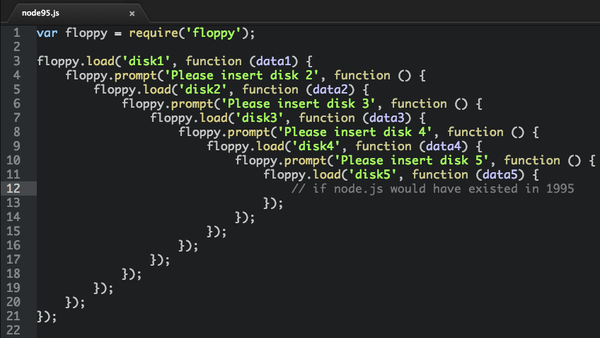
\includegraphics[width=0.75\paperwidth]{figures/functionsInFunctionsFail}
	\end{center}
\end{frame}

\begin{frame}[fragile]{Code Samples: Coroutines}
	\begin{center}
		
\includegraphics[width=0.5\paperwidth]{figures/functionsInFunctionsMeme}
	\end{center}
\end{frame}

\begin{frame}[fragile]{Code Samples: Coroutines}
	\begin{overlayarea}{\textwidth}{.6\textheight}
		\begin{columns}
			\begin{column}{0.5\textwidth}
				\begin{onlyenv}<1->
\textbf{OutOfMemoryError:}
\begin{lstlisting}[language=java,basicstyle=\ttfamily\tiny]
for (i in 1..100_000) {
  thread(start = true) {
    Thread.sleep(1000)
  }
}
\end{lstlisting}
\textbf{Works fine:}
\begin{lstlisting}[language=Kotlin,basicstyle=\ttfamily\tiny]
val jobs = List(100_000) {
  async(CommonPool) {
    delay(1000L)
    1
  }
}

runBlocking { // bridge async world
  println(jobs.sumBy {
    it.await()
  })
}
\end{lstlisting}
				\end{onlyenv}
			\end{column}
			\begin{column}{0.5\textwidth}
				\begin{onlyenv}<2->
					\begin{center}
						
\includegraphics[width=\textwidth]{figures/twoStatesEveryProgrammer}
					\end{center}
				\end{onlyenv}
			\end{column}
		\end{columns}
	\end{overlayarea}
\end{frame}

\begin{frame}[fragile]{Visibility And Modules}
	\begin{columns}
		\begin{column}{0.45\textwidth}
			Package-Level
			\begin{itemize}
				\item \textbf{public}\\
				is used by default\\
				declarations will be visible everywhere
				\item \textbf{private}\\
				only visible inside the file
				\item \textbf{protected}\\
				is not available for top-level declarations
				\item \textbf{internal}\\
				visible everywhere in the same module
			\end{itemize}
		\end{column}
		\begin{column}{0.55\textwidth}
			Class-Level
			\begin{itemize}
				\item \textbf{private}\\
				visible inside this class only
				\item \textbf{protected}\\
				same as private and visible in subclasses too
				\item \textbf{public}\\
				any client who sees the declaring\\
				class sees its public members
				\item \textbf{internal}\\
				any client inside this module\\
				who sees the declaring class\\
				sees its internal members
			\end{itemize}
		\end{column}
	\end{columns}
\end{frame}

\section{Traps \& Pitfalls}

\begin{frame}{Traps \& Pitfalls: Spring, Hibernate, \dots}
	\begin{itemize}
		\item Springs field injection does not work cause all fields are not null
		\begin{itemize}
			\item use "lateinit" on your @Autowired fields
			\item seriously use constructor injection over field injection
		\end{itemize}
		\item Classes are closed by default\\
		Spring can not proxy closed (final) classes
		\begin{itemize}
			\item use the "kotlin-allopen" maven/gradle plugin
			\item use the "kotlin-spring" maven/gradle plugin
		\end{itemize}
		\item Data classes have no non-argument constructor\\
		Hibernate/Jackson need non-argument constructor to create instances
		\begin{itemize}
			\item use the "kotlin-jpa" maven/gradle plugin
			\item use the "kotlin-noarg" maven/gradle plugin
		\end{itemize}
	\end{itemize}
\end{frame}

\begin{frame}[fragile]{Traps \& Pitfalls: Loopception}
	\begin{overlayarea}{\textwidth}{\textheight}
		\begin{onlyenv}<1->
\begin{lstlisting}[language=Kotlin,basicstyle=\ttfamily\small]
fun loopception() {
  for(i in 1..2) {
  print("$i")
    for (j in 3..4) {
      print("$j")
      if (j== 3) break
}}}

fun main(args: Array<String>) = loopception()
\end{lstlisting}
		\end{onlyenv}
		\begin{onlyenv}<2->
			\textbf{Outputs:} "1323"
		\end{onlyenv}
	\end{overlayarea}
\end{frame}

\begin{frame}[fragile]{Traps \& Pitfalls: Loopception}
	\begin{overlayarea}{\textwidth}{\textheight}
		\begin{onlyenv}<1->
\begin{lstlisting}[language=Kotlin,basicstyle=\ttfamily\small]
fun loopception() {
  outerLoop@ for(i in 1..2) {
  print("$i")
    for (j in 3..4) {
      print("$j")
      if (j == 3) break@outerLoop
}}}

fun main(args: Array<String>) = loopception()
\end{lstlisting}
		\end{onlyenv}
		\begin{onlyenv}<2->
			\textbf{Outputs:} "13"\\\vspace{\baselineskip}
		\end{onlyenv}
		\begin{onlyenv}<3->
			\textbf{return} \dots returns from the nearest enclosing function\\
			\textbf{break} \dots terminates the nearest enclosing loop\\
			\textbf{continue} \dots proceeds to the next step of the nearest enclosing loop
		\end{onlyenv}
	\end{overlayarea}
\end{frame}


\begin{frame}[fragile]{Traps \& Pitfalls: The return of power throw}
	\begin{overlayarea}{\textwidth}{.5\textheight}
		\begin{onlyenv}<1->
\begin{lstlisting}[language=Kotlin,basicstyle=\ttfamily\small]
fun powerThrow() {
  return throw throw return
}

fun main(args: Array<String>) = powerThrow()
\end{lstlisting}
		\end{onlyenv}
		\begin{onlyenv}<2->
			Yep it compiles\\
			return returns from the nearest enclosing function\\
			return itself returns type Nothing()
		\end{onlyenv}
	\end{overlayarea}
\end{frame}

\begin{frame}[fragile]{Traps \& Pitfalls: Almighty Type Inference}
	\begin{overlayarea}{\textwidth}{.6\textheight}
		\begin{onlyenv}<1->
\begin{lstlisting}[language=Kotlin,basicstyle=\ttfamily\small]
fun hello() = print("Hello")
fun world() = {
  print(" World")
}

fun main(args: Array<String>) {
  hello()
  world()
}	
\end{lstlisting}
		\end{onlyenv}
		\begin{onlyenv}<2->
			\textbf{Output:} "Hello"
		\end{onlyenv}
	\end{overlayarea}
\end{frame}

\begin{frame}[fragile]{Traps \& Pitfalls: Almighty Type Inference}
	\begin{overlayarea}{\textwidth}{.6\textheight}
		\begin{onlyenv}<1->
\begin{lstlisting}[language=Kotlin,basicstyle=\ttfamily\small]
fun hello(): Unit = print("Hello")
fun world(): () -> Unit = {
  print(" World")
}

fun main(args: Array<String>) {
  hello()
  world().invoke()
}
\end{lstlisting}
		\end{onlyenv}
		\begin{onlyenv}<2->
			\textbf{Output:} "Hello World"
		\end{onlyenv}
	\end{overlayarea}
\end{frame}

\section{Kotlin Native}

\begin{frame}[fragile]{Kotlin Native: GTK3}
	\textbf{Check it out:}\\\vspace{.5\baselineskip}
\begin{lstlisting}[language=bash,basicstyle=\ttfamily\small]
mkdir kotlin-native-samples && \
cd kotlin-native-samples && \
git init && \
git config core.sparseCheckout true && \
git remote add -f origin \
  https://github.com/JetBrains/kotlin-native.git && \
echo "samples/*" > .git/info/sparse-checkout && \
git checkout v0.3
\end{lstlisting}
\end{frame}

\begin{frame}[fragile]{Kotlin Native: GTK3}
	\textbf{Compile your first sample:}\\\vspace{.5\baselineskip}
\begin{lstlisting}[language=bash,basicstyle=\ttfamily\small]
docker run --rm -ti --workdir /sample -u root \
-v "$(pwd)/samples/gtk:/sample" \
hemeroc/kotlin-native:v0.3.0 \
/bin/bash -c \
"apt-get update; apt-get install libgtk-3-dev; ./build.sh"
\end{lstlisting}
	\textbf{Try it out:}\\\vspace{.5\baselineskip}
\begin{lstlisting}[language=bash,basicstyle=\ttfamily\small]
./samples/gtk/build/bin/Gtk3Demo.kexe
\end{lstlisting}
\end{frame}

\begin{frame}[fragile]{Kotlin Native: GTK3}
	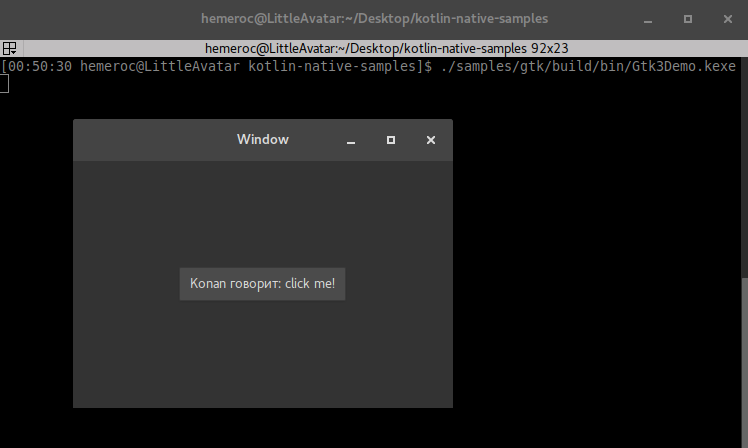
\includegraphics[width=0.85\paperwidth]{figures/gtk3}
\end{frame}

\section{Contribute \& Get Started}

{
	
\usebackgroundtemplate{
\includegraphics[height=\paperheight]{figures/kotlinLogo1Transparent}}

\begin{frame}{Contribute}
	\begin{center}
		\LARGE \href{https://youtrack.jetbrains.com/issues/KT/}{https://youtrack.jetbrains.com/issues/KT/}\\
		\href{https://github.com/Kotlin/KEEP}{https://github.com/Kotlin/KEEP}
	\end{center}
\end{frame}

\begin{frame}{Getting Started}
	\begin{center}
		\LARGE \href{https://kotlin.link/}{https://kotlin.link/}\\
		\href{http://slack.kotlinlang.org/}{http://slack.kotlinlang.org/}\\
		\href{https://github.com/Kotlin/kotlin-koans}{https://github.com/Kotlin/kotlin-koans}
	\end{center}
\end{frame}

\begin{frame}{Thank You}
	\begin{center}
		\LARGE Get started with\\
		\vspace{.5cm}
		
\includegraphics[width=.5\paperwidth]{figures/kotlinLogo2}\\
		\vspace{.5cm}
		\href{https://try.kotlinlang.org/}{https://try.kotlinlang.org/}
	\end{center}
\end{frame}

}